
\chapter{Implementation}

This chapter details the implementation of the methods mentioned before into a working system. The system consists of 2 main components, the frontend, consisting of the Javascript bookmarklet and the UI displaying the extracted data. This was impelemented in Ruby on Rails. The second component is the machine learning component, implemented in Java using the Weka library.

%diagram of the system architecture.

\section{Selection Interface}
\label{chap:selection}

The selection interface described in this section aims to provide visual feedback to the user when building a suitable wrapper for the page chosen by the user. The interface is implemented in the form of a bookmarklet which the user simply has to drag and drop into his/her browser toolbar. This bookmarklet can then be activated when the user reaches a page which he/she wants to have something extracted. Clicking on items will select them in green, and subsequent clicking will expand the scope of the extraction, with the items to be extracted highlighted in yellow. Figure \ref{fig:selection_example} shows a screenshot of a search result in bookdepository.co.uk with the bookmarklet activated.

\begin{figure}[htbp]
\centering
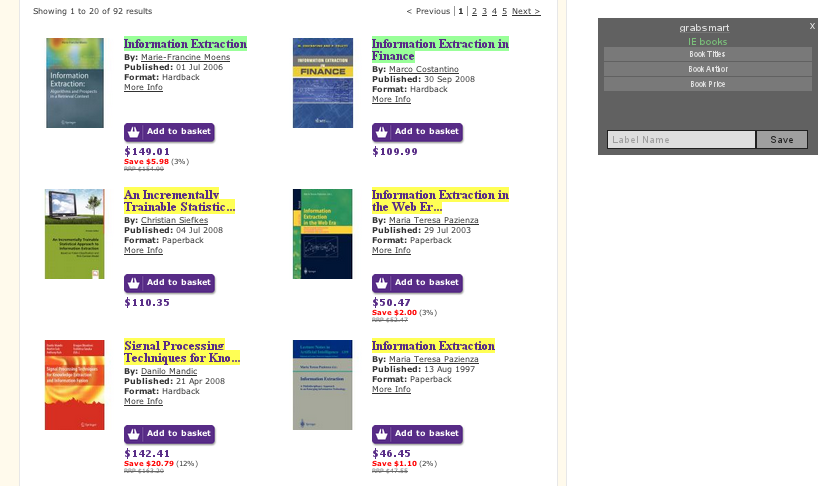
\includegraphics[scale=0.43]{selection_example.png} 
\caption{An example of the selection interface in action.}
\label{fig:selection_example}
\end{figure}

For greater automation, the bookmarklet interface attempts to reduce the amount of labelling work the user has to do by trying to predict what the user wants to extract from the page. More specifically, as the user selects the individual HTML elements on the page using the interface, the bookmarklet attempts to generalise an XPath that captures the selected elements, and also elements on the page with similar characteristics, like class names and position within the parent tag.

%have a loopy diagram to show the iterative work between user and algo.

The process is an iterative one. When the user clicks on a new element on the page, the XPath is recalculated, and then used to highlight the captured items on the page. This way, the user understands the changes he/she has made to the extraction scope as he/she clicks on additional items. The user is then able to perform this task for any number of labels the user thinks is appropriate for the extractor he/she is creating.

The bookmarklet does this by way of AJAX callbacks to the RoR frontend. One of the technical difficulties in implementing this was the fact that the standard XMLHttpRequest method of AJAX callbacks were not usable due to the cross-site security put into place by the Javascript API. The workaround was to use hidden form elements within the interface to send POST requests back to the server. Data was fetched by inserting script tags and callbacks to allow the JSON objects to be passed back into the small Javascript application.

\section{Machine Learning Component}
Once the XPath is sent from the bookmarklet back to the server-side application and inserted into the database, the user then has the option to test his/her created extractor. Once the user selects this option the machine-learning component visits the new page inserted, and crawls within the domain for similar pages. In this context, similar pages refer to HTML documents that return results, of any number, when a query is made using any of the previously labelled XPaths. 


\begin{figure}[htbp]
\centering

\tikzstyle{action}=[rectangle,
			thick,
			minimum size=1cm,	
			draw=gray!80,
			fill=gray!20]
\tikzstyle{ml}=[rectangle,
			thick,
			minimum size=1cm,	
			draw=red!80,
			fill=red!20]
\tikzstyle{background}=[rectangle,
			fill=gray!10,
			inner sep=0.15cm,
			rounded corners=2mm]

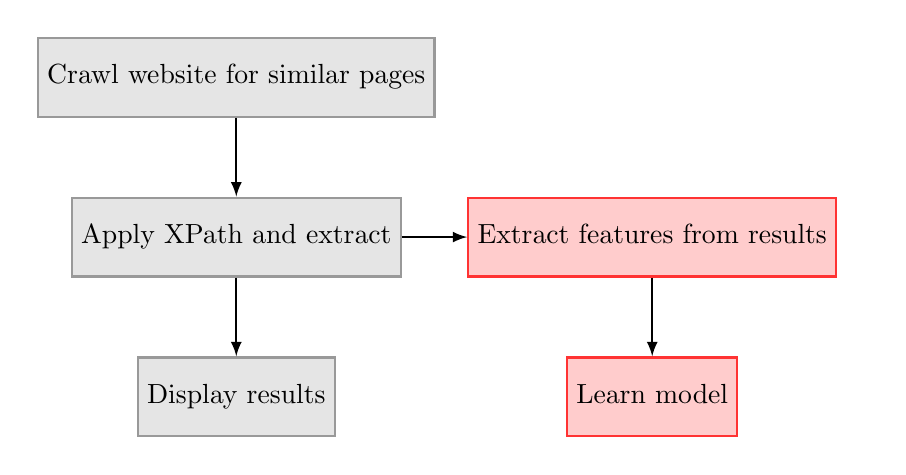
\begin{tikzpicture}[>=latex,text height=1.3ex,text depth=0.23ex]
  	\matrix[row sep=1cm,column sep=0.4cm]{
		\node (action1) [action]{Crawl website for similar pages}; 
		\\
		\node (action2) [action]{Apply XPath and extract}; &
		\node (ml1) [ml]{Extract features from results}; & 
		\\
		\node (action3) [action]{Display results}; &
		\node (ml2) [ml]{Learn model}; & 
		\\
	};
	\path[->]
	(action1) edge[thick] (action2)
	(action2) edge[thick] (action3)
	(action2) edge[thick] (ml1)
	(ml1)	edge[thick] (ml2)
	;
\end{tikzpicture}
\caption{Workflow of the machine learning component}
\label{fig:mlworkflow}
\end{figure}

	The extracted data is inserted back into the database, and then made available to the user. At the same time, features are extracted from this data in order to create a model for extraction for future use.
	
	